\documentclass{beamer}

\usetheme{Madrid}
\usecolortheme{dolphin}
\usepackage{graphicx}
\usepackage{tikz}
\usepackage{hyperref}
\usepackage{listings}

% Add JSON language support for listings
\definecolor{stringcolor}{RGB}{42,0.0,255}
\definecolor{keywordcolor}{RGB}{127,0,85}
\definecolor{numbercolor}{RGB}{0,0,0}

\lstdefinelanguage{json}{
    basicstyle=\normalfont\ttfamily,
    numbers=left,
    numberstyle=\scriptsize,
    stepnumber=1,
    numbersep=8pt,
    showstringspaces=false,
    breaklines=true,
    frame=lines,
    literate=
     *{0}{{{\color{numbercolor}0}}}{1}
      {1}{{{\color{numbercolor}1}}}{1}
      {2}{{{\color{numbercolor}2}}}{1}
      {3}{{{\color{numbercolor}3}}}{1}
      {4}{{{\color{numbercolor}4}}}{1}
      {5}{{{\color{numbercolor}5}}}{1}
      {6}{{{\color{numbercolor}6}}}{1}
      {7}{{{\color{numbercolor}7}}}{1}
      {8}{{{\color{numbercolor}8}}}{1}
      {9}{{{\color{numbercolor}9}}}{1}
      {:}{{{\color{keywordcolor}{:}}}}{1}
      {,}{{{\color{keywordcolor}{,}}}}{1}
      {\{}{{{\color{keywordcolor}{\{}}}}{1}
      {\}}{{{\color{keywordcolor}{\}}}}}{1}
      {[}{{{\color{keywordcolor}{[}}}}{1}
      {]}{{{\color{keywordcolor}{]}}}}{1}
      {"}{{{{\color{stringcolor}{"}}}}{1}
      {true}{{{\color{keywordcolor}{true}}}}{4}
      {false}{{{\color{keywordcolor}{false}}}}{5},
}

\title{Paper Bridge Finder}
\subtitle{Discovering Connections Between Research Areas}
\author{Your Name}
\institute{Your Institution}
\date{\today}

\begin{document}

\begin{frame}
    \titlepage
\end{frame}

\begin{frame}{Outline}
    \tableofcontents
\end{frame}

\section{Introduction}

\begin{frame}{The Challenge}
    \begin{itemize}
        \item Scientific literature is growing exponentially
        \item Research domains are increasingly specialized
        \item Finding connections between fields is difficult but valuable
        \item Manual exploration is time-consuming and limited
    \end{itemize}
    
    \vspace{0.5cm}
    \begin{center}
        \textbf{How can we automatically discover papers that connect different research areas?}
    \end{center}
\end{frame}

\begin{frame}{Paper Bridge Finder}
    \begin{columns}
        \column{0.6\textwidth}
        A system that:
        \begin{itemize}
            \item Ingests academic papers from repositories
            \item Clusters papers into research topics
            \item Builds a knowledge graph of papers and topics
            \item Identifies and ranks "bridge papers" between topics
            \item Provides explanations for why papers are bridges
        \end{itemize}
        
        \column{0.4\textwidth}
        \begin{center}
            % Replace missing image with a placeholder
            \fbox{
                \begin{minipage}{0.9\textwidth}
                    \centering
                    \textbf{[Knowledge Graph]}\\
                    \vspace{0.3cm}
                    \textit{Network visualization of papers and topics}
                \end{minipage}
            }
        \end{center}
    \end{columns}
\end{frame}

\section{System Architecture}

\begin{frame}{System Architecture}
    \begin{center}
        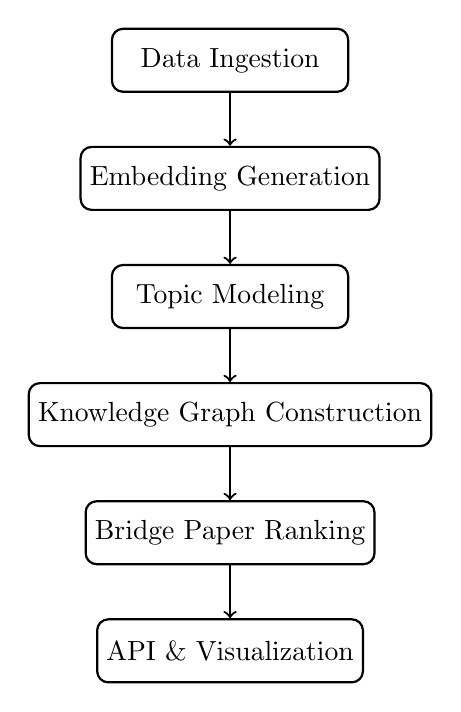
\begin{tikzpicture}[node distance=1.5cm, auto, thick]
            \node[draw, rectangle, rounded corners, minimum width=3cm, minimum height=0.8cm] (ingest) {Data Ingestion};
            \node[draw, rectangle, rounded corners, minimum width=3cm, minimum height=0.8cm, below of=ingest] (embed) {Embedding Generation};
            \node[draw, rectangle, rounded corners, minimum width=3cm, minimum height=0.8cm, below of=embed] (topic) {Topic Modeling};
            \node[draw, rectangle, rounded corners, minimum width=3cm, minimum height=0.8cm, below of=topic] (graph) {Knowledge Graph Construction};
            \node[draw, rectangle, rounded corners, minimum width=3cm, minimum height=0.8cm, below of=graph] (bridge) {Bridge Paper Ranking};
            \node[draw, rectangle, rounded corners, minimum width=3cm, minimum height=0.8cm, below of=bridge] (api) {API \& Visualization};
            
            \draw[->] (ingest) -- (embed);
            \draw[->] (embed) -- (topic);
            \draw[->] (topic) -- (graph);
            \draw[->] (graph) -- (bridge);
            \draw[->] (bridge) -- (api);
        \end{tikzpicture}
    \end{center}
\end{frame}

\begin{frame}{Data Ingestion}
    \begin{itemize}
        \item Sources: arXiv API and Semantic Scholar API
        \item Extracts paper metadata:
        \begin{itemize}
            \item Title, abstract, authors, publication year
            \item Citation information (when available)
        \end{itemize}
        \item Follows citation links to build a network
        \item Configurable "hop limit" to control exploration depth
    \end{itemize}
    
    \begin{lstlisting}[basicstyle=\tiny\ttfamily]
    python python/ingest.py --ids 2303.08774 2304.01852 --hops 1
    \end{lstlisting}
\end{frame}

\begin{frame}{Embedding Generation}
    \begin{itemize}
        \item Uses SentenceTransformer to create vector embeddings
        \item Model: \texttt{all-MiniLM-L6-v2}
        \item 384-dimensional vectors capture semantic meaning
        \item Enables similarity calculations and clustering
    \end{itemize}
    
    \begin{lstlisting}[basicstyle=\tiny\ttfamily]
    python python/embed.py
    \end{lstlisting}
\end{frame}

\begin{frame}{Topic Modeling}
    \begin{itemize}
        \item K-means clustering on normalized embeddings
        \item Automatically determines research topics
        \item Topic names generated from frequent terms
        \item Example topics:
        \begin{itemize}
            \item Topic 0: "chatgpt + models + large" (33 papers)
            \item Topic 1: "learning + transfer + deep" (41 papers)
        \end{itemize}
    \end{itemize}
    
    \begin{lstlisting}[basicstyle=\tiny\ttfamily]
    python python/topic_model_simple.py --n-clusters 3
    \end{lstlisting}
\end{frame}

\begin{frame}{Knowledge Graph Construction}
    \begin{columns}
        \column{0.6\textwidth}
        \begin{itemize}
            \item NetworkX graph with papers and topics as nodes
            \item Edge types:
            \begin{itemize}
                \item Paper-Topic (weight: 1.0)
                \item Citation (weight: 0.7)
                \item Same-Topic Similarity (weight: 0.5)
                \item Cross-Topic (weight: 0.3)
            \end{itemize}
            \item Cross-topic edges enable bridge discovery
        \end{itemize}
        
        \column{0.4\textwidth}
        \begin{center}
            % Replace missing image with a placeholder
            \fbox{
                \begin{minipage}{0.9\textwidth}
                    \centering
                    \textbf{[Graph View]}\\
                    \vspace{0.3cm}
                    \textit{Network visualization}
                \end{minipage}
            }
        \end{center}
    \end{columns}
    
    \begin{lstlisting}[basicstyle=\tiny\ttfamily]
    python python/graph.py
    \end{lstlisting}
\end{frame}

\begin{frame}{Bridge Paper Ranking}
    \begin{itemize}
        \item Identifies papers that connect different topics
        \item Scoring factors:
        \begin{itemize}
            \item Path distance: How efficiently the paper connects topics
            \item Centrality: Paper's importance in the overall graph
            \item Recency: More recent papers get higher weight
            \item Connection strength: Number and weight of connections
        \end{itemize}
        \item Provides explanations for why papers are bridges
    \end{itemize}
    
    \begin{equation*}
    score = \alpha \cdot (1/path\_length) + \beta \cdot centrality + \gamma \cdot recency + \delta \cdot connection\_strength
    \end{equation*}
\end{frame}

\section{Results}

\begin{frame}{Example Bridge Papers}
    \begin{table}
    \centering
    \small
    \begin{tabular}{p{1.8cm}p{5.5cm}p{1.2cm}p{1cm}}
    \hline
    \textbf{Paper ID} & \textbf{Title} & \textbf{Topics} & \textbf{Score} \\
    \hline
    2302.10205 & ChatIE: Zero-Shot Information Extraction via ChatGPT & 0 $\leftrightarrow$ 1 & 0.250 \\
    2303.03953 & ChatGPT: Beginning of an End of Manual Linguistic Data Annotation? & 0 $\leftrightarrow$ 1 & 0.243 \\
    1811.09751 & Characterizing and Avoiding Negative Transfer & 0 $\leftrightarrow$ 1 & 0.209 \\
    \hline
    \end{tabular}
    \end{table}
    
    \vspace{0.3cm}
    \begin{itemize}
        \item Bridge papers connect large language models with transfer learning
        \item They apply techniques from one domain to problems in another
        \item Provide pathways for interdisciplinary research
    \end{itemize}
\end{frame}

\begin{frame}{Case Study: ChatIE}
    \begin{columns}
        \column{0.6\textwidth}
        "ChatIE: Zero-Shot Information Extraction via ChatGPT" is a strong bridge because:
        \begin{itemize}
            \item Directly connected to Topic 0 (large language models)
            \item Methodologically connected to Topic 1 through zero-shot learning
            \item High centrality in the knowledge graph
            \item Recent publication (2023)
            \item Multiple connections to papers in both topics
        \end{itemize}
        
        \column{0.4\textwidth}
        \begin{center}
            % Replace missing image with a placeholder
            \fbox{
                \begin{minipage}{0.9\textwidth}
                    \centering
                    \textbf{[Bridge Paper]}\\
                    \vspace{0.3cm}
                    \textit{Visualization of paper connections}
                \end{minipage}
            }
        \end{center}
    \end{columns}
\end{frame}

\section{Implementation}

\begin{frame}{Pipeline Implementation}
    \begin{itemize}
        \item Unified pipeline script automates the entire workflow
        \item Command-line options for customization
        \item Skip individual steps if needed
        \item Start API server after processing
    \end{itemize}
    
    \begin{lstlisting}[basicstyle=\tiny\ttfamily]
    python python/pipeline.py --ids 2303.08774 2304.01852 --n-clusters 3 --start-api
    \end{lstlisting}
    
    \vspace{0.3cm}
    Technology stack:
    \begin{itemize}
        \item Python, NumPy, Pandas
        \item SentenceTransformer, scikit-learn
        \item NetworkX, FastAPI, Matplotlib
    \end{itemize}
\end{frame}

\section{Conclusion}

\begin{frame}{Strengths and Limitations}
    \begin{columns}
        \column{0.5\textwidth}
        \textbf{Strengths}
        \begin{itemize}
            \item Automated discovery of connections
            \item Scalable pipeline architecture
            \item Modular, extensible design
            \item Transparent explanations
            \item Visual exploration
        \end{itemize}
        
        \column{0.5\textwidth}
        \textbf{Limitations}
        \begin{itemize}
            \item Depends on metadata quality
            \item Limited by citation data
            \item Fixed number of topics
            \item Currently English-only
            \item Computational requirements
        \end{itemize}
    \end{columns}
\end{frame}

\begin{frame}{Applications and Future Work}
    \begin{columns}
        \column{0.5\textwidth}
        \textbf{Applications}
        \begin{itemize}
            \item Research discovery
            \item Literature review
            \item Research planning
            \item Educational use
            \item Interdisciplinary collaboration
        \end{itemize}
        
        \column{0.5\textwidth}
        \textbf{Future Work}
        \begin{itemize}
            \item Scalability improvements
            \item Advanced topic modeling
            \item User interface enhancements
            \item Integration with research tools
            \item Temporal analysis
        \end{itemize}
    \end{columns}
\end{frame}

\begin{frame}{Thank You}
    \begin{center}
        \Huge Thank you!
        
        \vspace{1cm}
        \large
        Questions?
    \end{center}
\end{frame}

\end{document} 